\documentclass[a4paper,12pt]{article}

\usepackage{geometry}
\usepackage{cmap}
\usepackage{enumerate}
\usepackage[russian]{babel}
\usepackage{hyperref}
\usepackage{listings}
\usepackage{verbatim}
\usepackage{pdfpages}
\usepackage[font=small,labelfont=bf]{caption}
\usepackage{float} 

\geometry{a4paper, left=20mm, right=10mm, top=20mm, bottom=20mm}

\lstdefinestyle{cppcode}{
	basicstyle=\ttfamily
}

\lstset{language=C++,style=cppcode}

\begin{document}

\begin{titlepage}		

\begin{center}
	\textsc{\textbf{Правительство Российской Федерации}}\\
	\vspace{0.5cm}
	\hrule
	\vspace{0.5cm}
	\textsc{Федеральное государственное автономное образовательное учреждение высшего образования <<Национальный исследовательский университет <<Высшая школа экономики>>}\\
	\vspace{1cm}
	Кафедра <<Компьютерная безопасность>>
\end{center}	

\vspace{\fill}

\begin{center}
	\Large{\textbf{ОТЧЕТ \\ К ЛАБОРАТОРНОЙ РАБОТЕ №2}} \\
	\vspace{1em}
	\textbf{по дисциплине} \\
	\vspace{1em}
	\large{\textbf{<<Языки программирования>>}}
\end{center}

\vspace{\fill}

\begin{flushright}
	\begin{minipage}[center]{15cm}
		\begin{minipage}[left]{5cm}
			{Работу выполнил\\студент группы СКБ-203}
		\end{minipage}
		\begin{minipage}[center]{5cm}
			\vspace{1.25cm}
			\hrulefill\\[-1cm]
			\begin{center}{подпись, дата}\end{center}
		\end{minipage}
		\begin{minipage}[right]{4cm}
			\vspace{0.4cm}
			\begin{flushright}{К.А. Павкин}\end{flushright}
		\end{minipage}
		\\
		\\
		\\
		\begin{minipage}[left]{5cm}
			{Работу проверил}
		\end{minipage}
		\begin{minipage}[center]{5cm}
			\vspace{1.25cm}
			\hrulefill\\[-1cm]
			\begin{center}{подпись, дата}\end{center}
		\end{minipage}
		\begin{minipage}[right]{4cm}
			\begin{flushright}{С.А. Булгаков}\end{flushright}
		\end{minipage}
	\end{minipage}
\end{flushright}

\vspace{\fill}

\begin{center}
	Москва~2021
\end{center}

\end{titlepage}

\tableofcontents
\thispagestyle{empty}
\cleardoublepage

\section*{<<Контейнер>>}\addcontentsline{toc}{section}{Постановка задачи}

Разработать программу на языке Си++ (ISO/IEC 14882:2014), демонстрирующую решение поставленной задачи.

\subsection*{Постановка задачи}

Разработать класс ADT и унаследовать от него классы, разработанные в рамках лабораторной работы 1.

Разработать набор классов, объекты которых реализуют типы данных, указанные ниже.
Для этих классов разработать необходимые конструкторы, деструктор, конструктор копирования.
Разработать операции: добавления/удаления элемента (уточнено в задаче); получения количества элементов; доступа к элементу (перегрузить оператор []).
При ошибках запускать исключение.

В главной функции разместить тесты, разработанные с использованием библиотеки GoogleTest.

\subsubsection*{Задачи}

\begin{enumerate}
	
\item
Динамический массив указателей на объекты ADT.
Размерность массива указателей увеличивается в момент его переполнения.
Начальная размерность задается как параметр конструктора, значение по умолчанию 0.
Добавление/удаление элемента в произвольное место.

\item
Стек, представленный динамическим массивом указателей на хранимые объекты ADT.
Размерность стека увеличивается в момент его переполнения.
Начальная размерность задается как параметр конструктора, значение по умолчанию 0.
Добавление/удаление элемента в начало и в конец.

\item
Односвязный список, содержащий указатели на объекты ADT.
Добавление/удаление элемента в произвольное место.

\item
Циклическая очередь, представленная динамическим массивом указателей на хранимые объекты ADT.
Добавление/удаление элемента в произвольное место.

\item
Двоичное дерево, содержащее указатели на объекты ADT.
Добавление/удаление элемента в произвольное место.

\end{enumerate}

\cleardoublepage

\section{Алгоритм решения задачи}

В процессе анализа предметной области были выявлены основные алгоритмы, необходимые для реализации всеобъемлющей, асимптотически эффективной и отлаженной программы для решения поставленной задачи.

На рисунке \ref{Class} представлена диаграмма классов, демонстрирующая формат хранения данных и зависимости между классами.
В целях сужения диаграммы без ущерба логике и смыслу были опущены закрытые служебные методы.

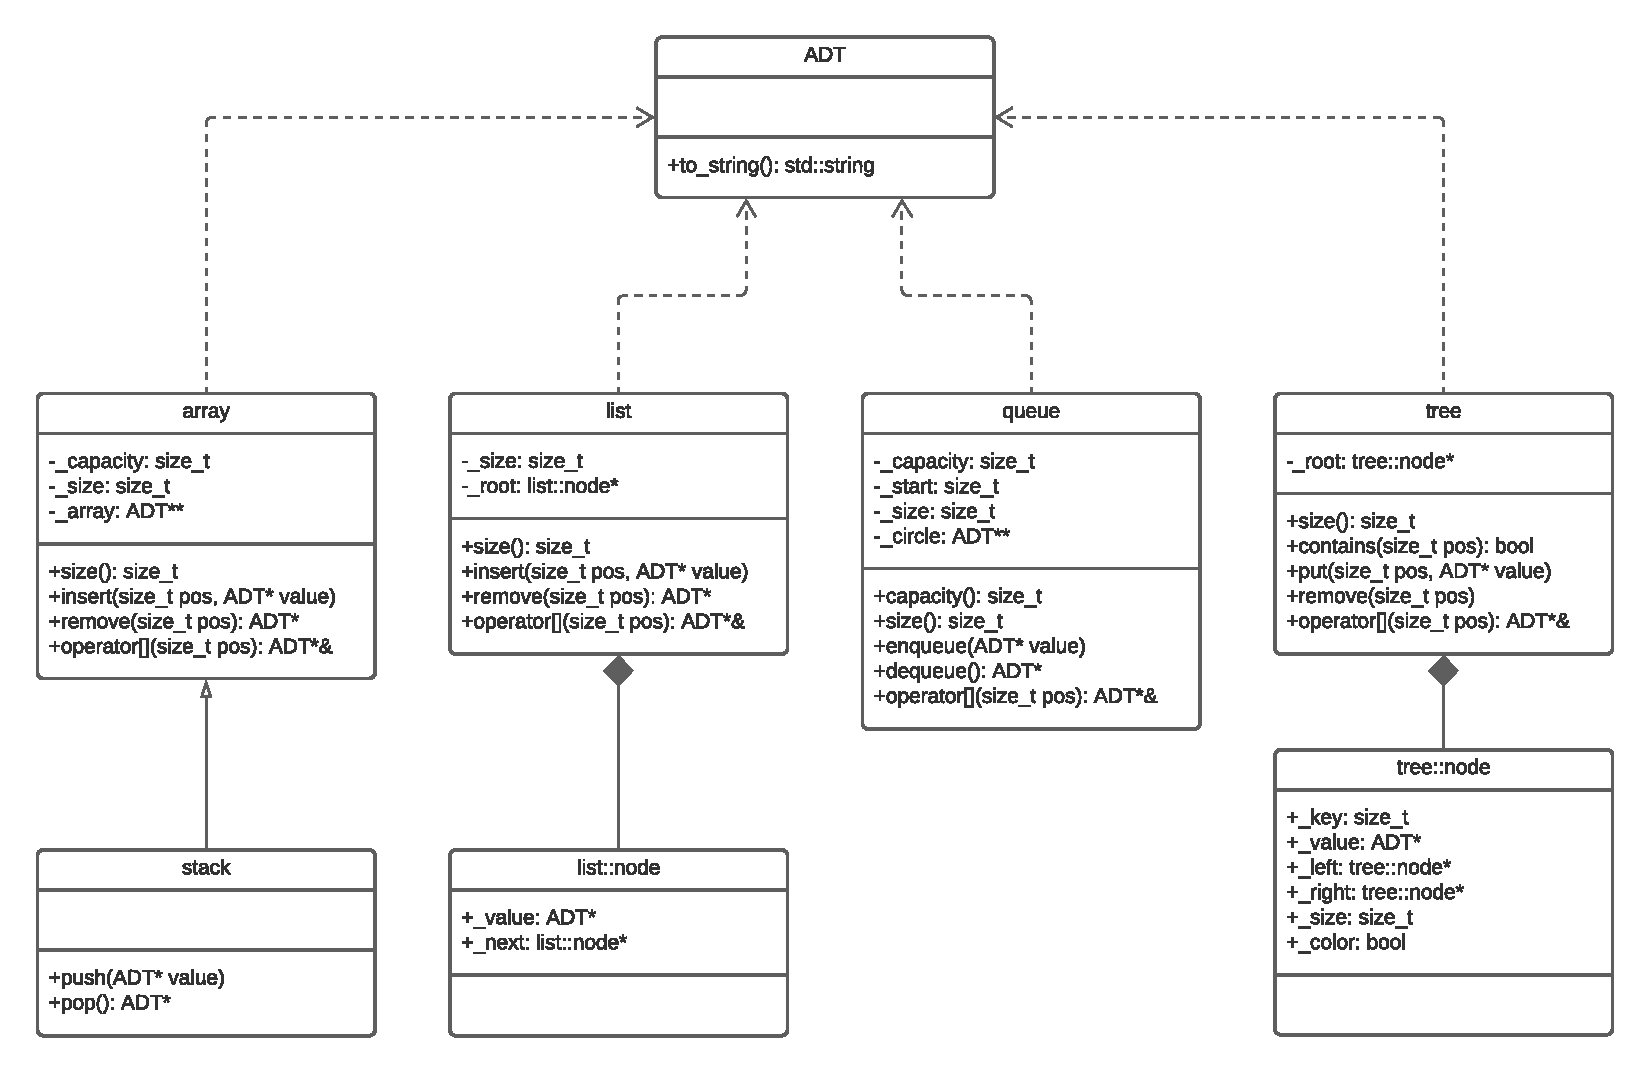
\includegraphics[width=\textwidth]{UML Class.pdf}

\captionof{figure}{Диаграмма классов}\label{Class}

\cleardoublepage

\subsection{Динамический массив}

В каноническом смысле, динамическим массивом называется контейнер, обладающий свойством расширяться и сжиматься в зависимости от количества заполненных элементов в нем.
При этом размерность ($capacity$) — фактически занимаемая массивом память — не превышает $2 * size$, где $size$ — количество непустых элементов в контейнере.
Такой подход позволяет добиться приемлимых затрат памяти при работе с неизвестным количеством входных данных.
Основные методы для работы с динамическим массивом и их асимптотическая сложность приведены в таблице \ref{comp1}.

\begin{table}[H]
	\caption{Методы класса array}
	\begin{center}
		\begin{tabular}{|l|l|c|}\hline\label{comp1}
			Название & Описание & Сложность \\ \hline
			\verb!insert! & Вставка элемента в произвольное место & $O(size)$ \\ \hline
			\verb!remove! & Удаление элемента из произвольного места & $O(size)$ \\ \hline
			\verb!operator[]! & Полулчение произвольного элемента & $O(1)$ \\ \hline
		\end{tabular}
	\end{center}
\end{table}

Здесь время вставки занимает в худшем случае $size$ операций, т. е. пропорционально количеству непустых элементов.
Однако, для случая вставки элемента в конец массива асимптотика будет несколько иная — $\Omega(1)$.
Так происходит потому, что операция вставки, при достижении конца контейнера, сопровождается выполнением закрытой процедуры \verb!resize! (листинг \ref{lst1}), которая увеличивает его размерность вдвое.

\begin{lstlisting}[caption={Процедура {\tt resize}},label=lst1]
	
void array::resize(size_t capacity)
{
	ADT** array = new ADT*[capacity];
	
	std::copy(_array, _array + std::min(_capacity, capacity), array);
	
	delete[] _array;
	
	_array = new ADT*[capacity];
	
	std::copy(array, array + capacity, _array);
	
	delete[] array;
	
	_capacity = capacity;
}
	
\end{lstlisting}

Аналогичным образом, при удалении элемента может вызываться процедура \verb!resize! в целях сужения массива, только уже втрое.
Это позволяет исключить ситуации с пороговым значением, при котором попеременные вставка и удаление элементов будут давать наихудшую производительность.

Полный код заголовочных файлов и файлов реализации динамического массива приведены в приложении А.

\subsubsection{Стек}

Стек, будучи наследуюемым от динамического массива, имеет ту же асимптотическую сложность и те же тонкости работы с ним.
Главное различие заключается в том, что операции вставки/удаления элементов стека ограничены лишь концом (по условию задачи и началом) контейнера.
Отрывок из файла реализации стека приведен в листинге \ref{lst2}.

\begin{lstlisting}[caption={Файл реализации стека},label=lst2]
	
	stack::stack(size_t capacity)
	: array(capacity)
	{
	}

	size_t stack::size() const
	{
		return array::size();
	}

	void stack::push(ADT* value)
	{
		array::insert(size(), value);
	}
	
	ADT* stack::pop()
	{
		return array::remove(size() - 1);
	}
	
	ADT*& stack::operator[](size_t pos)
	{
		return array::operator[](pos);
	}
	
\end{lstlisting}

Полный код заголовочных файлов и файлов реализации стека приведены в приложении Б.

\cleardoublepage

\subsection{Односвязный список}

В отличие от динамического массива, односвязный список занимает константное время для операций вставки/удаления элемента из начала или конца контейнера (в зависимости от реализации) при любых условиях.
Это становится возможным благодаря устройству односвязного списка, при котором среди закрытых переменных хранится <<корень>> — первый или последний элемент контейнера, в котором, помимо значения, находится также ссылка на следующий (предыдущий) элемент.
В листинге \ref{lst3} показан отрывок заголовочного файла для описания односвязного списка.

\begin{lstlisting}[caption={Отрывок заголовочного файла для описания односвязного списка},label=lst3]

class list {
	struct node {
		ADT* _value;
		node* _next;
		
		node(ADT*, node* = nullptr);
	};
	
	size_t _size;
	node* _root;

	// ...
};

\end{lstlisting}

Вставка/удаление элемента из односвязного списка происходит несколько быстрее, нежели аналогичное действие в динамическом массиве, поскольку отсутствуют издержки для заполнения и копирования контейнера.
Однако, асимптотическая сложность остается прежней — $O(size)$.
При больших объемах данных односвязный список также выигрывает у динамического массива, поскольку первый занимает место, пропорциональное количеству элементов в нем.

Основным недостатком данной реализации является время, необходимое для доступа к элементу контейнера по индексу, ведь для этого необходимо пройти все узлы вплоть до получаемого элемента.

Полный код заголовочных файлов и файлов реализации односвязного списка приведены в приложении В.

\cleardoublepage

\subsection{Циклическая очередь}

Будучи контейнером с константной размерностью, циклическая очередь не обеспечивает динамического расширения или сужения.
Её основное преимущество заключается в том, что все операции, по определению свойственные этому типу данных, занимают константное время.

Для обеспечения подобной функциональности достаточно поддерживать обычный массив, а также индексы начала и конца отрезка хранящихся в нем элементов.
В листинге \ref{lst4} показан отрывок заголовочного файла для описания циклической очереди.

\begin{lstlisting}[caption={Отрывок заголовочного файла для описания циклической очереди},label=lst4]

class queue {
	size_t _capacity, _start, _size;
	ADT** _circle;
	
	// ...
};

\end{lstlisting}

Можно заметить, что в представленной реализации вместо индекса, служащего обозначением конца очереди, используется переменная $size$.
Такой подход позволяет делать внутренние проверки без лишних вычислений.
Для получения конечной позиции заполненного отрезка достаточно взять остаток от деления суммы стартовой позиции $start$ и количества элементов контейнера $size$.

Полный код заголовочных файлов и файлов реализации односвязного списка приведены в приложении Г.

\cleardoublepage

\subsection{Бинарное дерево}

Наиболее подходящей с точки зрения надежности и эффективности реализацией бинарного дерева является так называемое красно-черное дерево.
Такое дерево идеально сбалансировано, и имеет асимтотическую сложность, не превышающую $O(\log_2 size)$ для всех необходимых операций (см. таблицу \ref{comp2}).

\begin{table}[H]
	\caption{Методы класса tree}
	\begin{center}
		\begin{tabular}{|l|l|c|}\hline\label{comp2}
			Название & Описание & Сложность \\ \hline
			\verb!put! & Вставка элемента в произвольное место & $O(\log_2 size)$ \\ \hline
			\verb!remove! & Удаление элемента из произвольного места & $O(\log_2 size)$ \\ \hline
			\verb!operator[]! & Полулчение произвольного элемента & $O(\log_2 size)$ \\ \hline
		\end{tabular}
	\end{center}
\end{table}

В отличие от классической реализации двоичного дерева поиска, красно-черное дерево может иметь помеченные (красные) ребра, которые говорят о том, что два узла, соединенные подобным ребром, можно рассматривать как один.
Это необходимо для того, чтобы размещать элементы не только слева и справа, как элементы с меньшими и большими ключами соответственно, но и между родственными.
Данное отличие как раз таки и позволяет достичь максимальной асимптотической эффективности для операции удаления элемента из произвольного места.
Представленный вариант бинарного дерева повсеместно используется для таких структур данных как <<множество>> или <<словарь>>.

В качестве хранимого значения выступает лишь одна переменная $root$, являющаяся экземпляром вложенного класса \verb!node!.
Этот класс содержит в себе: ключ, однозначно идентифицирующий положение элемента в дереве, значение, ссылки на левый и правый потомки, размер поддерева и цвет ребра, ведущего к родительскому узлу.
В листинге \ref{lst5} показан отрывок заголовочного файла для описания бинарного дерева.

\begin{lstlisting}[caption={Отрывок заголовочного файла для описания бинарного дерева},label=lst5]

class tree {
	struct node {
		K _key;
		ADT* _value;
		node* _left;
		node* _right;
		size_t _size;
		bool _color;
		
		node(K, ADT*, size_t, bool);
	};
	
	node* _root;
	
	// ...
};

\end{lstlisting}

Так, при вставке/удалении элемента может потребоваться смещение некоторых узлов дерева (балансировка) ради сохранения эффективности последующих операций.
Это обеспечивается, главным образом, благодаря функциям смещения поддерева влево или вправо (см. листинг \ref{lst6}).
	
\begin{lstlisting}[caption={Функция смещения поддерева влево},label=lst6]

template <typename K>
typename tree<K>::node* tree<K>::rotate_left(node* n)
{
	node* temp = n->_right;
	n->_right = temp->_left;
	temp->_left = n;
	temp->_color = temp->_left->_color;
	temp->_left->_color = RED;
	temp->_size = n->_size;
	n->_size = size(n->_left) + size(n->_right) + 1;
	
	return temp;
}

\end{lstlisting}

Полный код заголовочных файлов и файлов реализации бинарного дерева приведены в приложении Д.

\cleardoublepage

\section{Получение исполняемых модулей}

Заголовочные файлы и их реализации были размещены в различных директориях.
Для сборки проекта в каждую директорию были помещены файлы CMakeLists.txt, и, таким образом, каждая директория представляет из себя отдельную библиотеку, которая в последствии собирается в корневом каталоге.
Файл сборки CMakeLists.txt из корневого каталога показан в листинге \ref{CMakeLists}.

\begin{lstlisting}[caption={Файл сборки CMakeLists.txt},label=CMakeLists]

cmake_minimum_required(VERSION 3.0)

project(laboratory-work-02-kapavkin)

set(CMAKE_CXX_STANDARD 14)

include(FetchContent)
FetchContent_Declare(
googletest
URL https://github.com/google/googletest/archive/609281088cfefc76f9d0
ce82e1ff6c30cc3591e5.zip
)

set(gtest_force_shared_crt ON CACHE BOOL "" FORCE)
FetchContent_MakeAvailable(googletest)

set(MAIN main.cpp)

enable_testing()

add_executable(main ${MAIN})

add_subdirectory(laboratory-work-01-kapavkin)
add_subdirectory(array)
add_subdirectory(list)
add_subdirectory(queue)
add_subdirectory(tree)

target_link_libraries(main
	laboratory-work-01-kapavkin
	array
	list
	queue
	tree
	gtest_main
)

include(GoogleTest)
gtest_discover_tests(main)


\end{lstlisting}

\cleardoublepage

\section{Тестирование}

Файл \verb!main.cpp! содержит юнит-тесты, целью которых является сравнение ожидаемых от функций значений с фактическими, и выдача оповещений при их несовпадении.

\subsection{Прецеденты класса {\tt array}}

Тестовые случаи для проверки корректности работы методов класса {\tt array}.

\begin{enumerate}

\item
\verb!constructor! — проверяет корректность конструкторов/деструкторов.

\item
\verb!insert! — проверяет корректность вставки элемента в произвольное место.

\item
\verb!remove! — проверяет корректность удаления элемента из произвольного места.

\end{enumerate}

\subsection{Прецеденты класса {\tt stack}}

Тестовые случаи для проверки корректности работы методов класса {\tt stack}.

\begin{enumerate}

\item
\verb!constructor! — проверяет корректность конструкторов/деструкторов.

\item
\verb!push! — проверяет корректность вставки элемента в конец стека.

\item
\verb!pop! — проверяет корректность удаления элемента из конца стека.

\end{enumerate}

\subsection{Прецеденты класса {\tt list}}

Тестовые случаи для проверки корректности работы методов класса {\tt list}.

\begin{enumerate}

\item
\verb!constructor! — проверяет корректность конструкторов/деструкторов.

\item
\verb!insert! — проверяет корректность вставки элемента в произвольное место.

\item
\verb!remove! — проверяет корректность удаления элемента из произвольного места.

\end{enumerate}

\subsection{Прецеденты класса {\tt queue}}

Тестовые случаи для проверки корректности работы методов класса {\tt queue}.

\begin{enumerate}

\item
\verb!constructor! — проверяет корректность конструкторов/деструкторов.

\item
\verb!enqueue! — проверяет корректность вставки элемента в конец очереди.

\item
\verb!dequeue! — проверяет корректность удаления элемента из начала очереди.

\item
\verb!oversize! — проверяет корректность при переполнении очереди.

\end{enumerate}

\subsection{Прецеденты класса {\tt tree}}

Тестовые случаи для проверки корректности работы методов класса {\tt tree}.

\begin{enumerate}
	
\item
\verb!constructor! — проверяет корректность конструкторов/деструкторов.

\item
\verb!put! — проверяет корректность вставки элемента в произвольное место.

\item
\verb!remove! — проверяет корректность удаления элемента из произвольного места.

\end{enumerate}

\cleardoublepage

\addcontentsline{toc}{section}{Приложения}

\section*{\begin{center} Приложение А \end{center}}\label{AA}

\subsection*{А.1 Заголовочный файл класса array}\label{AA1}

\verbatiminput{../array/array.h}
\cleardoublepage

\subsection*{А.2 Файл реализации класса array}\label{AA2}

\verbatiminput{../array/array.cpp}
\cleardoublepage

\section*{\begin{center} Приложение Б \end{center}}\label{AB}

\subsection*{Б.1 Заголовочный файл класса stack}\label{AB1}

\verbatiminput{../array/stack/stack.h}
\cleardoublepage

\subsection*{Б.2 Файл реализации класса stack}\label{AB2}

\verbatiminput{../array/stack/stack.cpp}
\cleardoublepage

\section*{\begin{center} Приложение В \end{center}}\label{AC}

\subsection*{В.1 Заголовочный файл класса list}\label{AC1}

\verbatiminput{../list/list.h}
\cleardoublepage

\subsection*{В.2 Файл реализации класса list}\label{AC2}

\verbatiminput{../list/list.cpp}
\cleardoublepage

\section*{\begin{center} Приложение Г \end{center}}\label{AD}

\subsection*{Г.1 Заголовочный файл класса queue}\label{AD1}

\verbatiminput{../queue/queue.h}
\cleardoublepage

\subsection*{Г.2 Файл реализации класса queue}\label{AD2}

\verbatiminput{../queue/queue.cpp}
\cleardoublepage

\section*{\begin{center} Приложение Д \end{center}}\label{AE}

\subsection*{Д.1 Заголовочный файл класса tree}\label{AE1}

\verbatiminput{../tree/tree.h}
\cleardoublepage

\subsection*{Д.2 Файл реализации класса tree}\label{AE2}

\verbatiminput{../tree/tree.cpp}
\cleardoublepage

\end{document}